% Created 2019-09-20 Fri 18:38
% Intended LaTeX compiler: pdflatex
\documentclass[xetex]{beamer}
\usepackage[utf8]{inputenc}
\usepackage[T1]{fontenc}
\usepackage{graphicx}
\usepackage{grffile}
\usepackage{longtable}
\usepackage{wrapfig}
\usepackage{rotating}
\usepackage[normalem]{ulem}
\usepackage{amsmath}
\usepackage{textcomp}
\usepackage{amssymb}
\usepackage{capt-of}
\usepackage{hyperref}
\usepackage{fontspec}
\setsansfont{Montserrat Regular}
\usetheme{Montpellier}
\usecolortheme{dove}
\usefonttheme{professionalfonts}
\author{Bruce Rannala}
\date{}
\title{EVE 231: Principles of Biological Data Analysis (Fall 2019)}
\hypersetup{
 pdfauthor={Bruce Rannala},
 pdftitle={EVE 231: Principles of Biological Data Analysis (Fall 2019)},
 pdfkeywords={},
 pdfsubject={},
 pdfcreator={Emacs 26.3 (Org mode 9.1.9)}, 
 pdflang={English}}
\begin{document}

\maketitle
\begin{frame}{Outline}
\tableofcontents
\end{frame}


\section{UNIX}
\label{sec:orgb4078c5}
\begin{frame}[label={sec:org5ccfe16}]{Early History}
\begin{itemize}
\item 1969. Ken Thompson, Dennis Ritchie and others started developing UNIX on the "little-used PDP-7 in a corner" at Bell Labs
\end{itemize}
\begin{center}
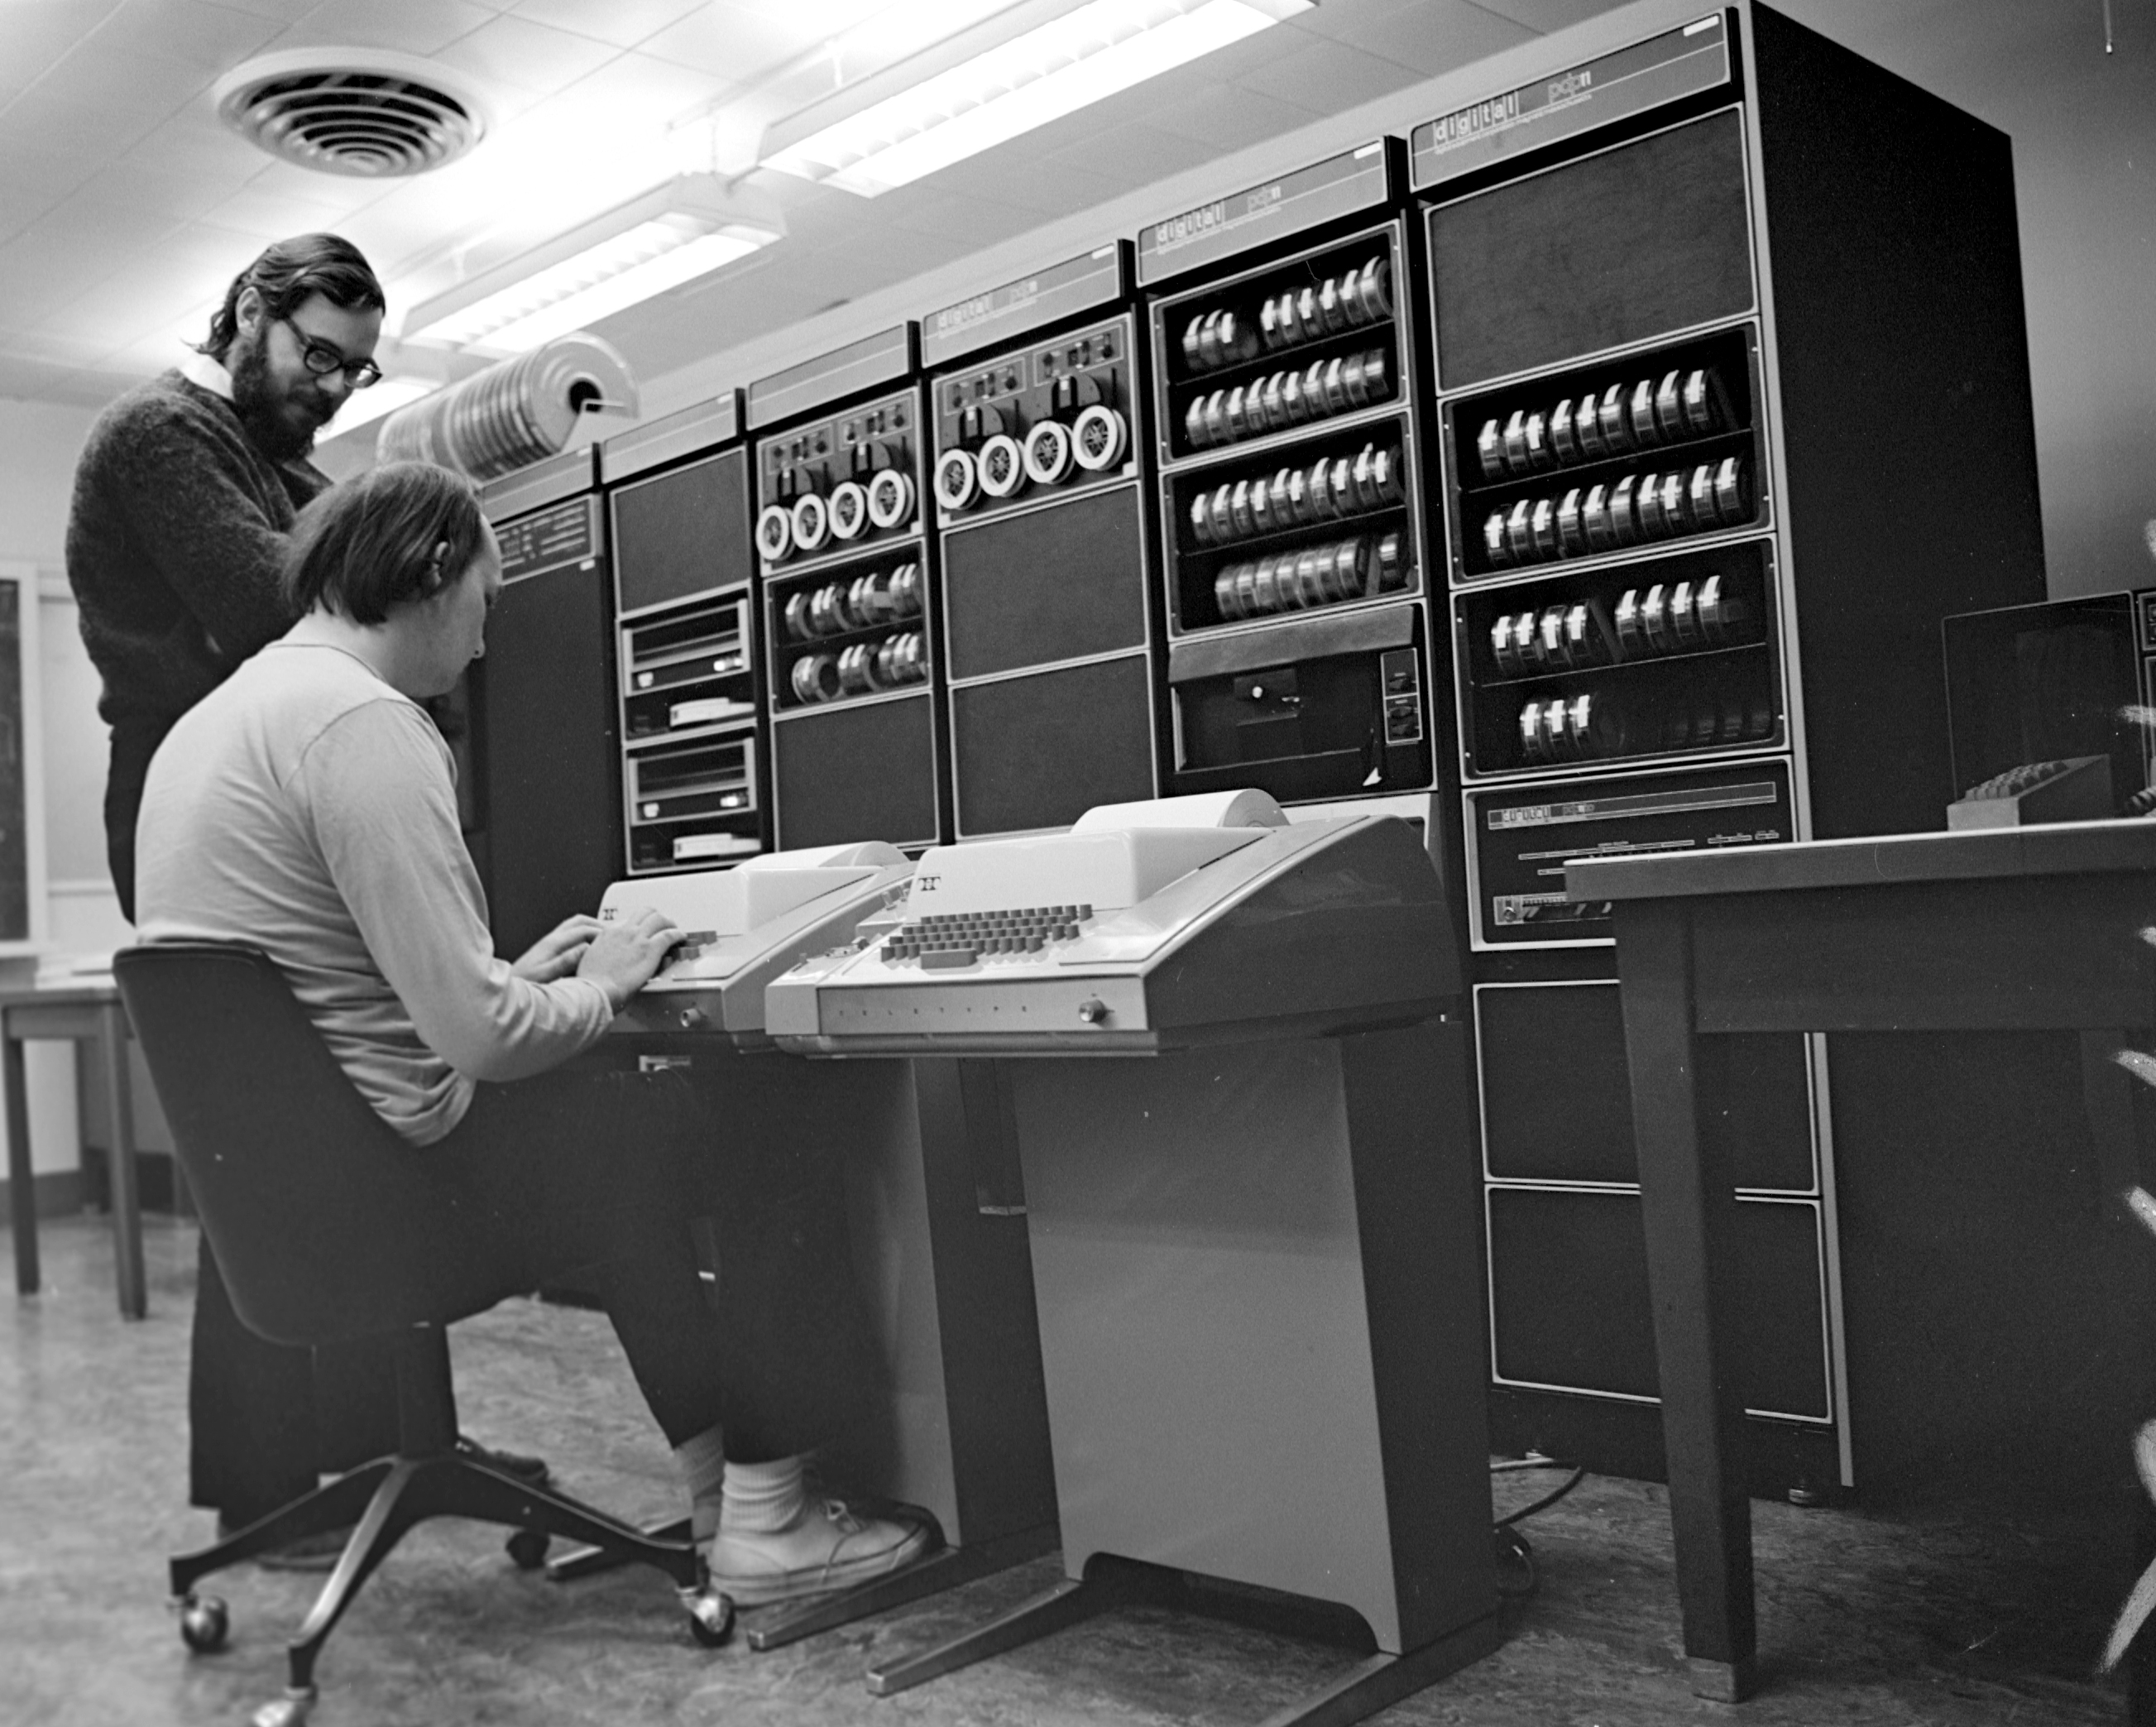
\includegraphics[width=0.25\textwidth]{./figs/ThompsonRitchieatPDP-11.jpg}
\end{center} 
\begin{itemize}
\item 1985. Free Software Foundation (GNU) founded by Richard Stallman
\item 1988. Portable Operating System Interface (POSIX) standards for UNIX introduced
\end{itemize}
\end{frame}
\begin{frame}[label={sec:orgf99f574}]{Early History (cont)}
\begin{itemize}
\item 1988 Free Software Foundation creates Copyleft Licence GNU General Public License (GNU GPL)
\item GPL guarantees end users the freedom to run, study, share and modify the software
\item GNU = ``GNUs Not Unix'' software is developed by the FSF and includes GCC compiler, Emacs and others
\end{itemize}
\end{frame}
\begin{frame}[label={sec:org375f1ec}]{Recent History}
\begin{itemize}
\item 1991. Linus Torvalds completes first Linux kernel.
\end{itemize}
\begin{center}
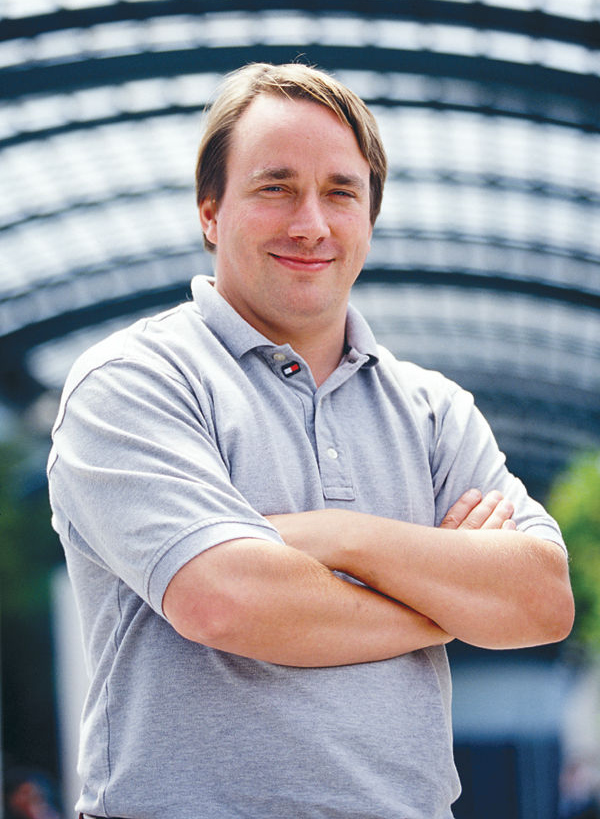
\includegraphics[width=0.15\textwidth]{./figs/Linus_Torvalds.jpeg}
\end{center} 
\begin{itemize}
\item 1992/1993 GNU software embedded into Linux to create GNU/Linux
\item 1994 Slackware Linux distribution released
\item 2000 Mac OS X public beta "Kodiak" released
\end{itemize}
\end{frame}
\begin{frame}[label={sec:org4a70513}]{UNIX Philosophy}
\begin{itemize}
\item Write programs that do one thing and do it well
\item Write programs to work together
\item Write programs to handle text streams, because that is a universal interface
\end{itemize}
\end{frame}
\end{document}